\lecture{13}{}{}

\begin{definition}
    Let G be a group. A Cayley digraph $C = (V, E)$ is a directed graph where $V = G$ and $E = \{(g, g \cdot a) : g \in G, a \in A\}$\\
    Where A is a generating set of G.\\
\end{definition}

\begin{eg}
    Let $G = \mathbb{Z}_8 = \{0, 1, 2, \cdots, 7\}$\\
    Let $S = \{2, 5\}$\\
    The Cayley digraph for $G$ with $S$ is shown below.\\
\end{eg}
\begin{answer}
    \vphantom{}\\
    \begin{center}
        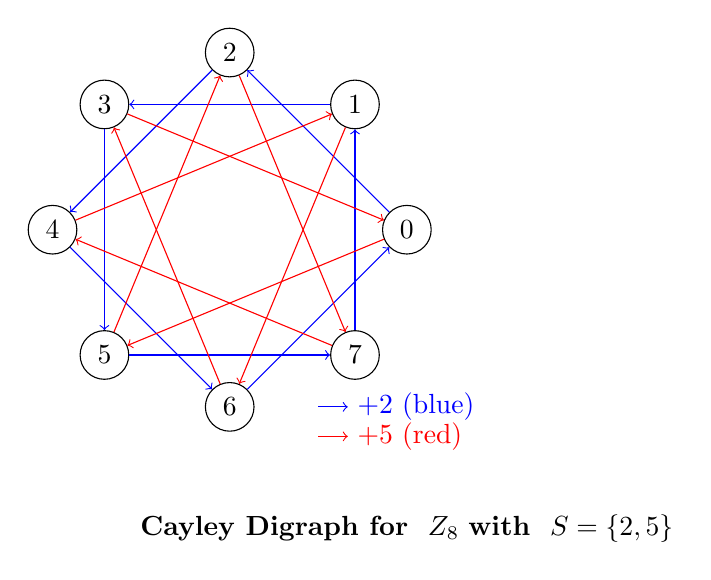
\begin{tikzpicture}[scale=0.75]
            % Define the vertices in a circle
            \foreach \i in {0,...,7} {
                \node[circle, draw, minimum size=0.5cm] (\i) at (360/8 * \i:3cm) {\i}; % Adjust node size here
            }
        
            % Define the directed edges for generator 2
            \foreach \i in {0,...,7} {
                \pgfmathtruncatemacro{\j}{mod(\i+2,8)}
                \draw[->, blue] (\i) -- (\j);
            }
        
            % Define the directed edges for generator 5
            \foreach \i in {0,...,7} {
                \pgfmathtruncatemacro{\j}{mod(\i+5,8)}
                \draw[->, red] (\i) -- (\j);
            }
            
            % Add legend
            \node[below=3.5cm] at (0) {\textbf{Cayley Digraph for } $Z_8$ \textbf{with } $S = \{2, 5\}$};
            \draw[blue,->] (1.5, -3) -- ++(0.5,0) node[right] {+2 (blue)};
            \draw[red,->] (1.5, -3.5) -- ++(0.5,0) node[right] {+5 (red)};
            
        \end{tikzpicture}
    \end{center}
\end{answer}

\chapter{Structure \& Groups}

\section{Groups of Permutations}

\begin{theorem}[Cayley's Theorem]
    Every group is isomorphic to a group of permutations.\\
\end{theorem}

\begin{eg}
    Roots of unity. Let $\omega = e^{\frac{2\pi i}{n}}$\\
    \[U_6 = \{1, \omega, \omega^2, \omega^3, \omega^4, \omega^5\}\]
    \[U_3 = \{1, \omega^2, \omega^4\}\]

    \noindent It is obvious that there is no isomorphism between $U_6$ and $U_3$.\\
    But we can define a homomorphism $\phi : U_6 \rightarrow U_3$\\
\end{eg}
\begin{answer}
    We can define $\phi : U_6 \rightarrow U_3$ by $\phi(\omega) = \omega^{2}$\\
    Let $z1, z2 \in U_6$\\
    \[\phi(z1 \cdot z2) = (z1 \cdot z2)^2 = z1^2 \cdot z2^2 = \phi(z1) \cdot \phi(z2)\]
\end{answer}